\documentclass[aspectratio=169]{beamer} % 16:9 widescreen (matches 13.333in x 7.5in)

\usetheme{moloch}

\usepackage[T1]{fontenc}
\usepackage[default]{opensans}

\usepackage{graphicx}
\usepackage{xcolor}
\usepackage{tikz}

% -----------------------
% Company color palette
% -----------------------
\definecolor{CompanyMain}{HTML}{00B6DF}
\definecolor{CompanyMainLight}{HTML}{CBF0F6}
\definecolor{CompanyAccent}{HTML}{FF5F25}
\definecolor{CompanyAccentLight}{HTML}{FFB7A1}
\definecolor{CompanyWhite}{HTML}{FFFFFF}
\definecolor{CompanyBlack}{HTML}{000000}
\newcommand{\CompanyConferenceLine}{Society for Laboratory Automation \& Screening - Boston, MA}
\newcommand{\DefaultVerticalSlideContentAlignment}{t} % t or c typically
% Force slide background to pure white (and normal text to black)
\setbeamercolor{background canvas}{bg=CompanyWhite}
\setbeamercolor{normal text}{fg=CompanyBlack,bg=CompanyWhite}

% Optional: remove navigation symbols
\setbeamertemplate{navigation symbols}{}

% -----------------------
% Logo file paths (SET THESE)
% -----------------------
\newcommand{\CompanyTitleLogoFile}{assets/title-logo}
\newcommand{\CompanyFooterLogoFile}{assets/footer-logo}

% -----------------------
% Footer knobs (tweak these) - using your current values
% -----------------------
\newlength{\CompanyFooterLogoHeight}
\setlength{\CompanyFooterLogoHeight}{4.5ex} % main knob: footer logo size

\newlength{\CompanyFooterPadV}
\setlength{\CompanyFooterPadV}{0.4ex} % knob: vertical padding inside the footer bar

\newlength{\CompanyFooterBarHeight}

\newlength{\CompanyFooterLeftPad}
\setlength{\CompanyFooterLeftPad}{0.7em} % knob: space between left edge and logo

\newlength{\CompanyFooterRightPad}
\setlength{\CompanyFooterRightPad}{0.7em} % knob: right padding inside footer bar

\newlength{\CompanyFooterNumberPad}
\setlength{\CompanyFooterNumberPad}{0.6em} % knob: extra space after slide number

% Recompute bar height from logo height + padding.
\newcommand{\CompanyFooterRecalc}{%
  \setlength{\CompanyFooterBarHeight}{\CompanyFooterLogoHeight}%
  \addtolength{\CompanyFooterBarHeight}{\CompanyFooterPadV}%
  \addtolength{\CompanyFooterBarHeight}{\CompanyFooterPadV}%
}

% Helper: vertically center content inside a fixed height box (used in the footer)
\newcommand{\CompanyVCenter}[2]{% #1 = height, #2 = content
  \vbox to #1{\vfil\hbox{#2}\vfil}%
}

% -----------------------
% Special "flush-left bullet" list
% IMPORTANT:
% - Use normal itemize for normal indentation (bullets under a paragraph).
% - Use FlushWithFrameTitleItemize ONLY when you want the BULLET to align with the left edge of normal slide text.
%
% Where to edit if bullets are too far left:
% - Increase \CompanyFlushLeftMargin (moves the whole flush-left list right).
% - Or increase \CompanyFlushLabelWidth (more space reserved for the bullet).
% -----------------------
\newlength{\CompanyFlushLeftMargin}
\setlength{\CompanyFlushLeftMargin}{1em} % KNOB: move flush-left bullets right (try 0.5em)

\newlength{\CompanyFlushLabelWidth}
\setlength{\CompanyFlushLabelWidth}{0.5em} % KNOB: reserved width for the bullet box

\newlength{\CompanyFlushLabelSep}
\setlength{\CompanyFlushLabelSep}{0em} % KNOB: space between bullet and text

\newenvironment{FlushWithFrameTitleItemize}[1][<+->]{%
  \begingroup
  \beamerdefaultoverlayspecification{#1}%
  \begin{list}{\usebeamertemplate{itemize item}}{%
    \setlength{\leftmargin}{\CompanyFlushLeftMargin}%
    \setlength{\labelwidth}{\CompanyFlushLabelWidth}%
    \setlength{\labelsep}{\CompanyFlushLabelSep}%
    \setlength{\itemindent}{0em}%
    % Left-align the label inside its box so the bullet does NOT "hang" into the margin.
    \def\makelabel##1{##1\hfil}%
  }%
}{%
  \end{list}%
  \endgroup
}

% -----------------------
% Frame title background (white / no solid color bar)
% Align the title flush with the body text block.
% -----------------------
\setbeamercolor{frametitle}{bg=CompanyWhite,fg=CompanyBlack}
\setbeamercolor{framesubtitle}{bg=CompanyWhite,fg=CompanyBlack}

% Frametitle padding knobs - using your current values
\newlength{\CompanyFrameTitlePadV}
\setlength{\CompanyFrameTitlePadV}{0.30cm} % vertical padding above and below the title

\newlength{\CompanyFrameTitlePadH}
\setlength{\CompanyFrameTitlePadH}{-2.6em} % horizontal padding inside title box (0pt = aligned to body)

\makeatletter
\setbeamertemplate{frametitle}{%
  \nointerlineskip
  \hbox{%
    % Place the title box starting exactly at the body text left margin
    \hspace*{\beamer@leftmargin}%
    \begin{beamercolorbox}[%
      wd=\textwidth,
      sep=0pt,
      leftskip=\CompanyFrameTitlePadH,
      rightskip=0pt
    ]{frametitle}%
      \vskip\CompanyFrameTitlePadV
      \usebeamerfont{frametitle}\insertframetitle\par
      \ifx\insertframesubtitle\empty%
      \else%
        \vskip0.15cm
        {\usebeamerfont{framesubtitle}\usebeamercolor[fg]{framesubtitle}\insertframesubtitle\par}%
      \fi%
      \vskip\CompanyFrameTitlePadV
    \end{beamercolorbox}%
  }%
}
\makeatother

% -----------------------
% Title page layout: top half white with logo, bottom half CompanyMain with text
% -----------------------
\setbeamertemplate{title page}{%
  \begin{tikzpicture}[remember picture,overlay]
    % Top half (CompanyWhite)
    \fill[CompanyWhite]
      (current page.north west)
      rectangle ([yshift=-0.5\paperheight]current page.north east);

    % Bottom half (CompanyMain)
    \fill[CompanyMain]
      (current page.south west)
      rectangle ([yshift=0.5\paperheight]current page.south east);

    % Title-slide logo (top-center)
    \node[anchor=north] at ([yshift=-1.1cm]current page.north) {%
      \includegraphics[height=2cm]{\CompanyTitleLogoFile}%
    };

    % Text block (bottom half)
    \node[anchor=south] at ([yshift=0.5cm]current page.south) {%
      \begin{minipage}{0.90\paperwidth}
        \centering
        {\color{CompanyWhite}\usebeamerfont{title}\inserttitle\par}
        \vspace{0.35cm}
        {\color{CompanyWhite}\usebeamerfont{author}\insertauthor\par}
        {\color{CompanyWhite}\usebeamerfont{institute}\insertinstitute\par}
                % Conference line (edit \CompanyConferenceLine above)
        \vspace{2ex}
        {\color{CompanyWhite}\usebeamerfont{institute}\CompanyConferenceLine\par}

        \vspace{0.15cm}
        {\color{CompanyWhite}\usebeamerfont{date}\insertdate\par}
      \end{minipage}
    };
  \end{tikzpicture}%
}

% -----------------------
% Footer bar: CompanyMain background, small logo left, slide number right (white)
% Keeps the logo vertically centered as it scales.
% -----------------------
\setbeamercolor{companyfooter}{bg=CompanyMain,fg=CompanyWhite}

\setbeamertemplate{footline}{%
  \CompanyFooterRecalc%
  \begin{beamercolorbox}[
    wd=\paperwidth,
    ht=\CompanyFooterBarHeight,
    dp=0pt,
    leftskip=0pt,
    rightskip=0pt
  ]{companyfooter}%
    \vbox to \CompanyFooterBarHeight{%
      \vfil
      \hbox to \paperwidth{%
        \hspace*{\CompanyFooterLeftPad}%
        \CompanyVCenter{\CompanyFooterLogoHeight}{%
          \includegraphics[height=\CompanyFooterLogoHeight]{\CompanyFooterLogoFile}%
        }%
        \hfill
        \CompanyVCenter{\CompanyFooterLogoHeight}{%
          \usebeamerfont{page number in head/foot}\insertframenumber%
        }%
        \hspace*{\CompanyFooterNumberPad}%
        \hspace*{\CompanyFooterRightPad}%
      }%
      \vfil
    }%
  \end{beamercolorbox}%
}

% Section slide that looks like content slides (and keeps the footer)
\AtBeginSection{%
  \begin{frame}
    \vfill
    \centering
    {\usebeamerfont{title}\insertsectionhead\par}
    \vfill
  \end{frame}
}

% -----------------------
% Metadata
% -----------------------
\title{Streamlining Automated Laboratory Workflows in Tightly Firewalled Networks}
\author{Eli Fine, PhD}
%\institute{Some University}
\date{February 10, 2026}

\begin{document}

% Title slide: no footer
{
\setbeamertemplate{footline}{}
\begin{frame}[plain,noframenumbering]
  \titlepage
\end{frame}
}

%\section{Introduction}

\begin{frame}[\DefaultVerticalSlideContentAlignment]
  \frametitle{Firewalls are Closing In}
  \pause
  \begin{FlushWithFrameTitleItemize}[<+->]
    \item Unfettered access to SaaS is going away
    \item Outbound connections are blocked, not just inbound---reverse shell attacks
    \item More sophisticated attack strategies are leading to restrictions in R\&D
    \item Automation inroads into Manufacturing; tighter restrictions or true air-gap
    \item Even company-hosted services sometimes blocked by `catch-all' IT policies
  \end{FlushWithFrameTitleItemize}
  % \begin{overlayarea}{\textwidth}{0.70\textheight}
  %   \only<+>{\includegraphics[height=0.70\textheight,keepaspectratio]{assets/overlay-1.png}}
  %   \only<+>{\includegraphics[height=0.70\textheight,keepaspectratio]{assets/overlay-2.png}}
  %   \only<+>{\includegraphics[height=0.70\textheight,keepaspectratio]{assets/overlay-3.png}}
  %   % Add more layers (no numbering needed):
  %   % \only<+>{\includegraphics[height=0.70\textheight,keepaspectratio]{assets/overlay-4.png}}
  % \end{overlayarea}

    \begin{overlayarea}{\textwidth}{0.65\textheight}
    \only<3->{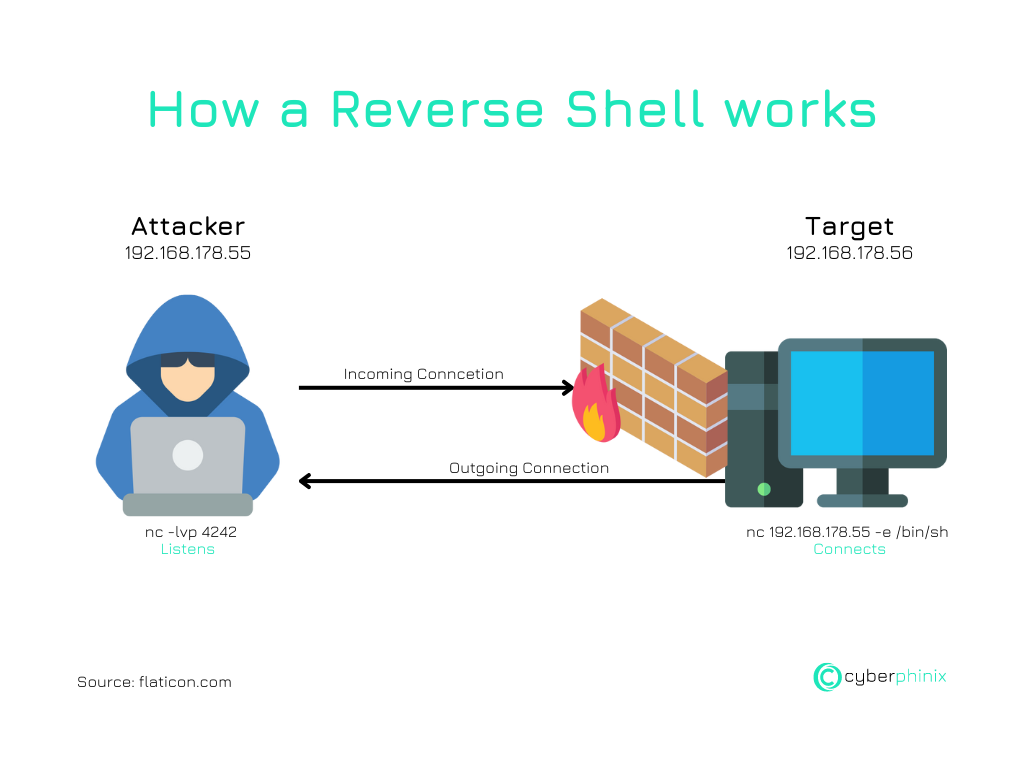
\includegraphics[height=0.65\textheight,keepaspectratio]{assets/How-a-Reverse-Shell-works.png}}
    
  \end{overlayarea}
  
\end{frame}


\begin{frame}[\DefaultVerticalSlideContentAlignment]
  \frametitle{Challenges with Notifications/Alerting}
  \pause
  \begin{FlushWithFrameTitleItemize}[<+->]
    \item Many instruments and software only send alerts via email
    \item Allowed mechanisms evolve as IT policies change
  \begin{FlushWithFrameTitleItemize}[<+->]
    \item Firewall rules to reach SaaS alerting (e.g. PagerDuty, Slack)
    \item Enterprise system operating within air-gapped enclave
  \end{FlushWithFrameTitleItemize}

    \item Many disparate lab systems/software to update to match new approach
  \end{FlushWithFrameTitleItemize}

    \vskip2ex\begin{overlayarea}{\textwidth}{0.35\textheight}
    \only<2->\hspace{2cm}{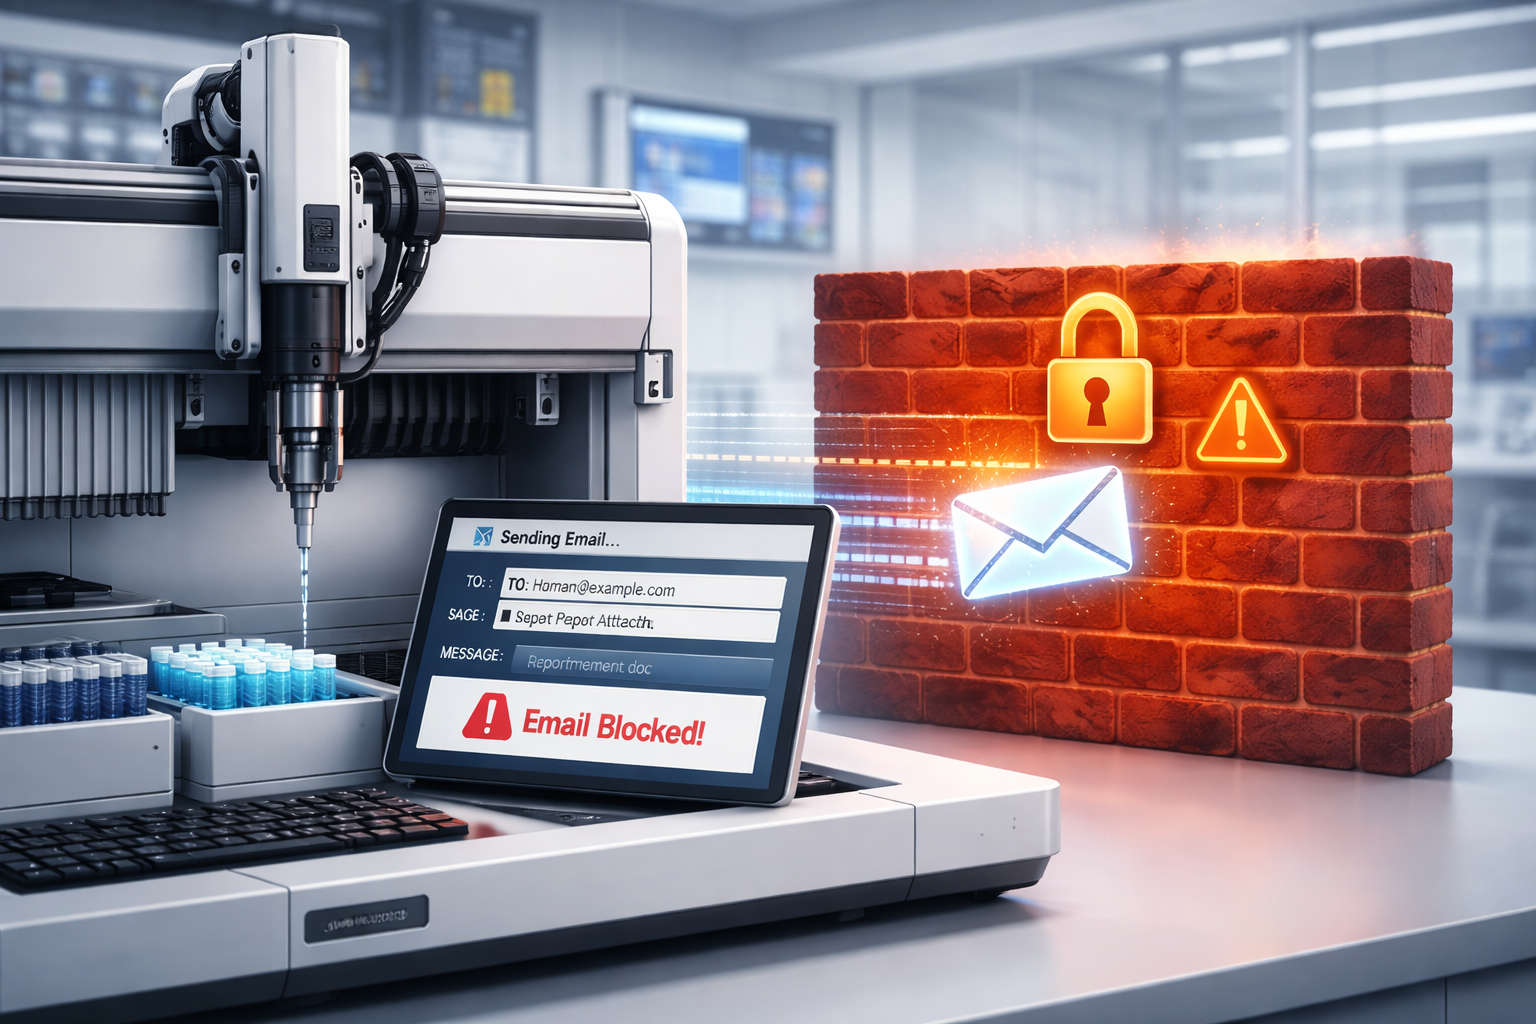
\includegraphics[height=0.35\textheight,keepaspectratio]{assets/email-block.png}}
    
  \end{overlayarea}
  
\end{frame}

\begin{frame}[\DefaultVerticalSlideContentAlignment]
  \frametitle{Challenges Using a Simulation Environment}
  \pause
  \begin{FlushWithFrameTitleItemize}[<+->]
    \item Simple scripts to copy/paste files over the network are blocked
    \item Vendor tools to `snapshot' workcells become cumbersome at scale
    \item Access to cloud-based version control (e.g. GitHub) is blocked
  \end{FlushWithFrameTitleItemize}  
\end{frame}

\begin{frame}[\DefaultVerticalSlideContentAlignment]
  \frametitle{Challenges Implementing Version Control}
  \pause
  \begin{FlushWithFrameTitleItemize}[<+->]
    \item 2-factor auth into corporate Git servers challenging while wearing PPE
    \item Cloud-based SaaS or corporate Git servers may be blocked by the firewall
    \item Many automation users unfamiliar with Git
  \end{FlushWithFrameTitleItemize}  
\end{frame}

\begin{frame}[\DefaultVerticalSlideContentAlignment]
  \frametitle{What does a solution need to accomplish?}
  \pause
  \begin{FlushWithFrameTitleItemize}[<+->]
    \item Observability
      \begin{FlushWithFrameTitleItemize}[<+->]
        \item Aggregate alerts from various sources (including email)
        \item Single touchpoint for reconfiguring forwarding alerts to new endpoints
      \end{FlushWithFrameTitleItemize}  
    
    \item Traceability
      \begin{FlushWithFrameTitleItemize}[<+->]
        \item Enable version control in the lab
        \item Easily transfer version history to/from simulation environment
        %\item Handle differences in files between lab and simulation environment
        \item Avoid complicated authentication while in PPE
        \item Require full authentication for critical steps
        \item Be user-friendly for people with limited experience using Git
      \end{FlushWithFrameTitleItemize}  
   \item Be compatible with Windows 10/11 (and Linux)
        
  \end{FlushWithFrameTitleItemize}  
\end{frame}

%\section{Approach}

\begin{frame}[\DefaultVerticalSlideContentAlignment]
  \frametitle{System Design Requirements}
  \pause
  \begin{FlushWithFrameTitleItemize}[<+->]

        \item Orchestrated lab with 10+ workcells and hundreds of devices
    
        \item Open-source, to facilitate security scanning \& review 
        % \item No `administrative' privileges needed for any applications
        \item Prefer containerized applications when possible to enhance compatibility
        \item Avoid Docker Desktop licensing concerns
        %\item Background services, not triggered by logon
        %\item API-first design to facilitate custom interactions
        \item Browser-based UIs to be accessible from anywhere on the network
      \end{FlushWithFrameTitleItemize}  
\end{frame}


\begin{frame}[\DefaultVerticalSlideContentAlignment]
  \frametitle{Setting up Host Computer to run Containers}
  \pause
  \begin{FlushWithFrameTitleItemize}[<+->]
    \item Windows 10, Windows 11, or Linux
    \item Transfer zip file with Rancher Desktop installer and applications
    \item Run install script (no PowerShell needed)
    \item Data from all applications in single location to enable easy backup

  \end{FlushWithFrameTitleItemize}
  
    \only<6->{\vskip2ex\begin{overlayarea}{\textwidth}{0.35\textheight}
    \hspace{2cm}{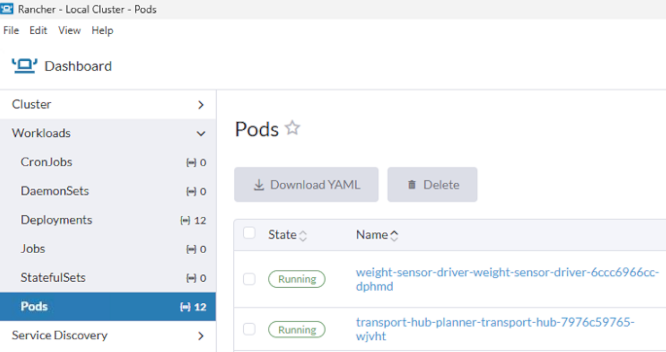
\includegraphics[height=0.35\textheight,keepaspectratio]{assets/rancher.png}}
    
  \end{overlayarea}}
  
\end{frame}

\begin{frame}[\DefaultVerticalSlideContentAlignment]
  \frametitle{Observability Architecture}
  
  \begin{columns}[T,onlytextwidth]
    % Left side: bullet list
    \begin{column}{0.35\textwidth}
        \begin{FlushWithFrameTitleItemize}[<+(1)->]
            \item Mailpit provides an email address to receive notifications
            \item Notifications can be sent via email or directly via API calls to the Nexus Notifications Center
        
            \item User interface accessible anywhere in lab
          \end{FlushWithFrameTitleItemize}
  \end{column}

    % Right side: graphic
    \begin{column}{0.65\textwidth}
      \vspace{0pt} % helps top-align the graphic with the left column
      \centering
      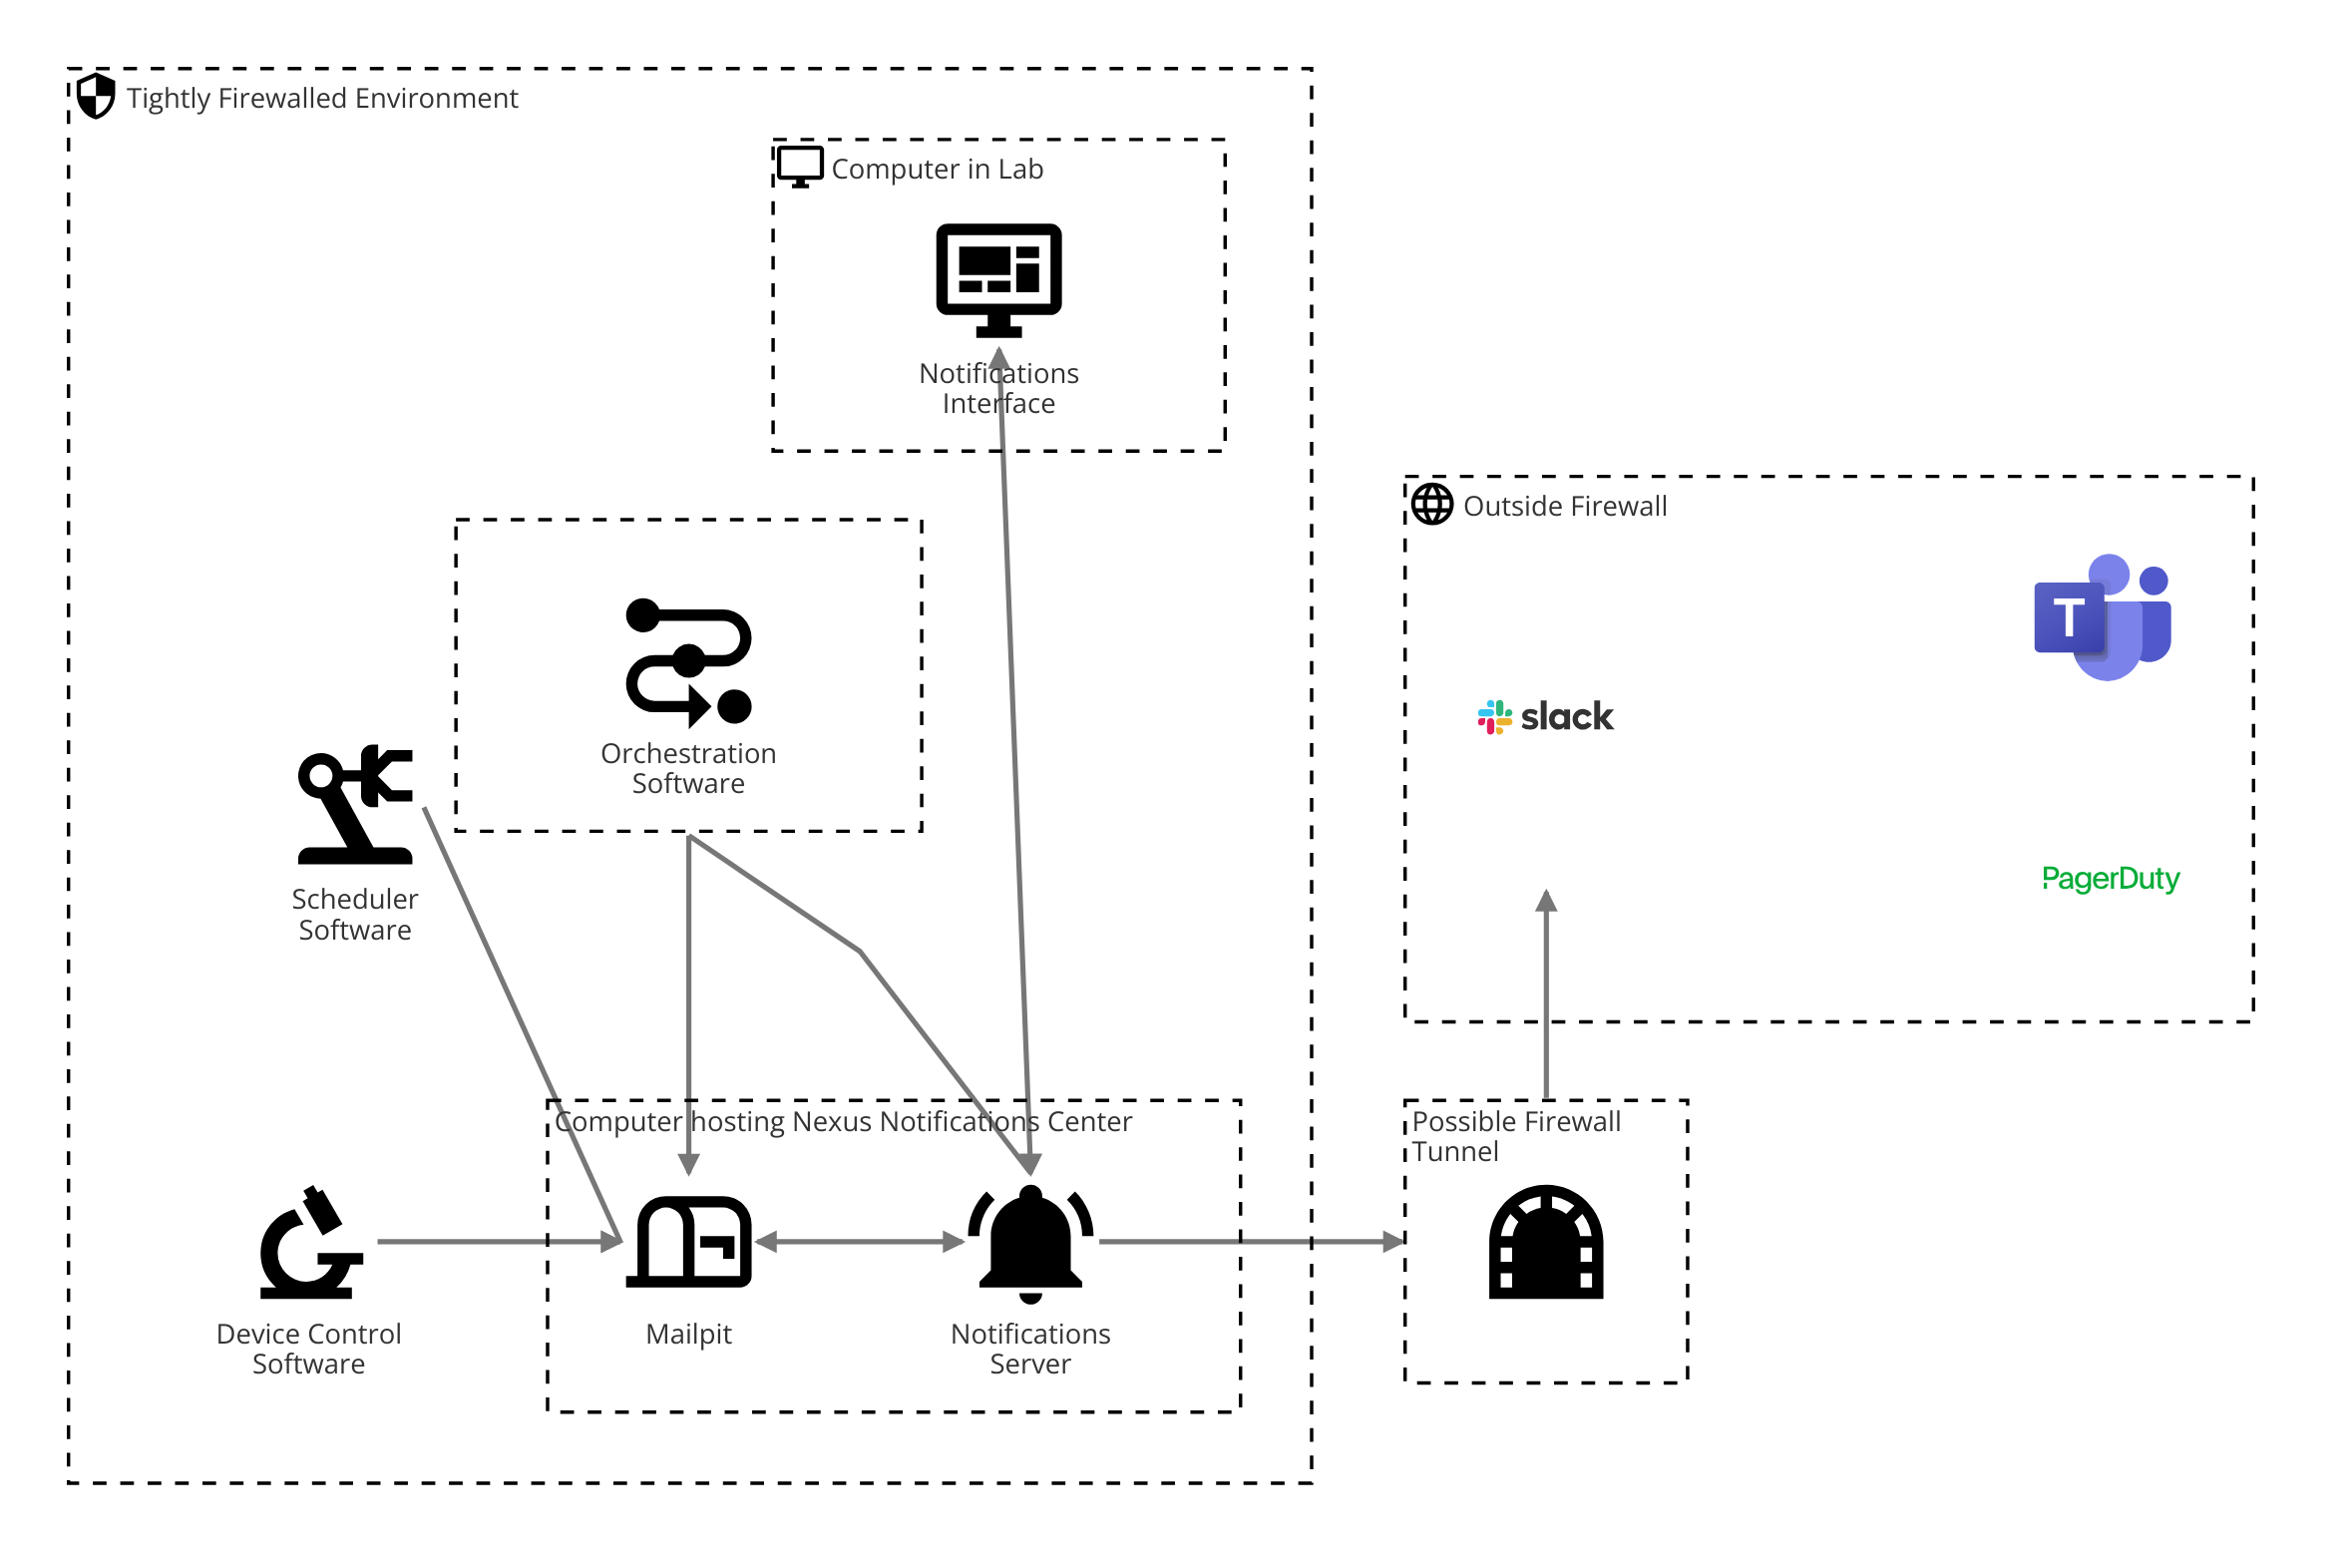
\includegraphics[width=\linewidth,keepaspectratio]{assets/nexus-architecture.png}
      % If you want a fixed height instead, use:
      % \includegraphics[height=0.62\textheight,keepaspectratio]{assets/my-graphic}
    \end{column}
  \end{columns}

\end{frame}

\begin{frame}[\DefaultVerticalSlideContentAlignment]
  \frametitle{Observability Dashboard --- Nexus Notifications Center}
  
    \vskip2ex\begin{overlayarea}{\textwidth}{0.65\textheight}
    \hspace{2cm}{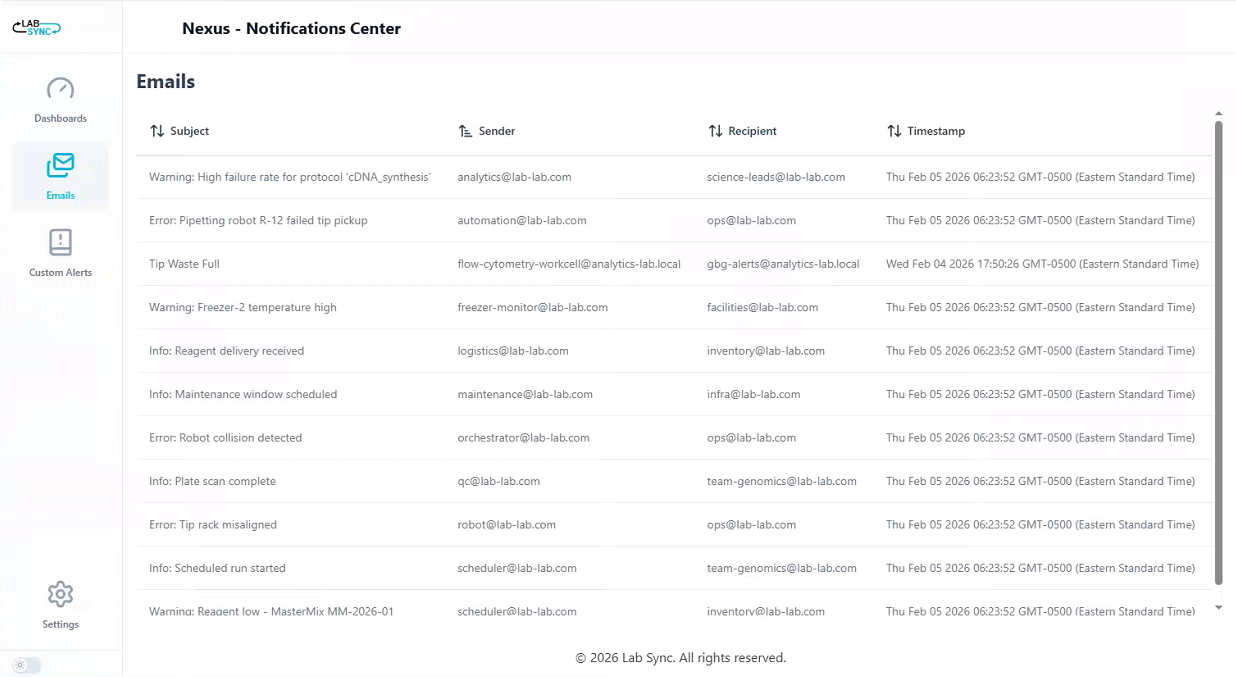
\includegraphics[height=0.65\textheight,keepaspectratio]{assets/notifications-light.png}} 
    
  \end{overlayarea}
  
\end{frame}

\begin{frame}[\DefaultVerticalSlideContentAlignment]
  \frametitle{Version Control Architecture}
  

  \begin{columns}[T,onlytextwidth]
    % Left side: bullet list
    \begin{column}{0.35\textwidth}
        \begin{FlushWithFrameTitleItemize}[<+(1)->]
            \item Gitea runs as a Git Server within the lab
            \item `Git Sherpa': purpose-built app to guide users through Git
            \item Git Bundles move changes across the boundary
          \end{FlushWithFrameTitleItemize}
  \end{column}

    % Right side: graphic
    \begin{column}{0.65\textwidth}
      \vspace{0pt} % helps top-align the graphic with the left column
      \centering
      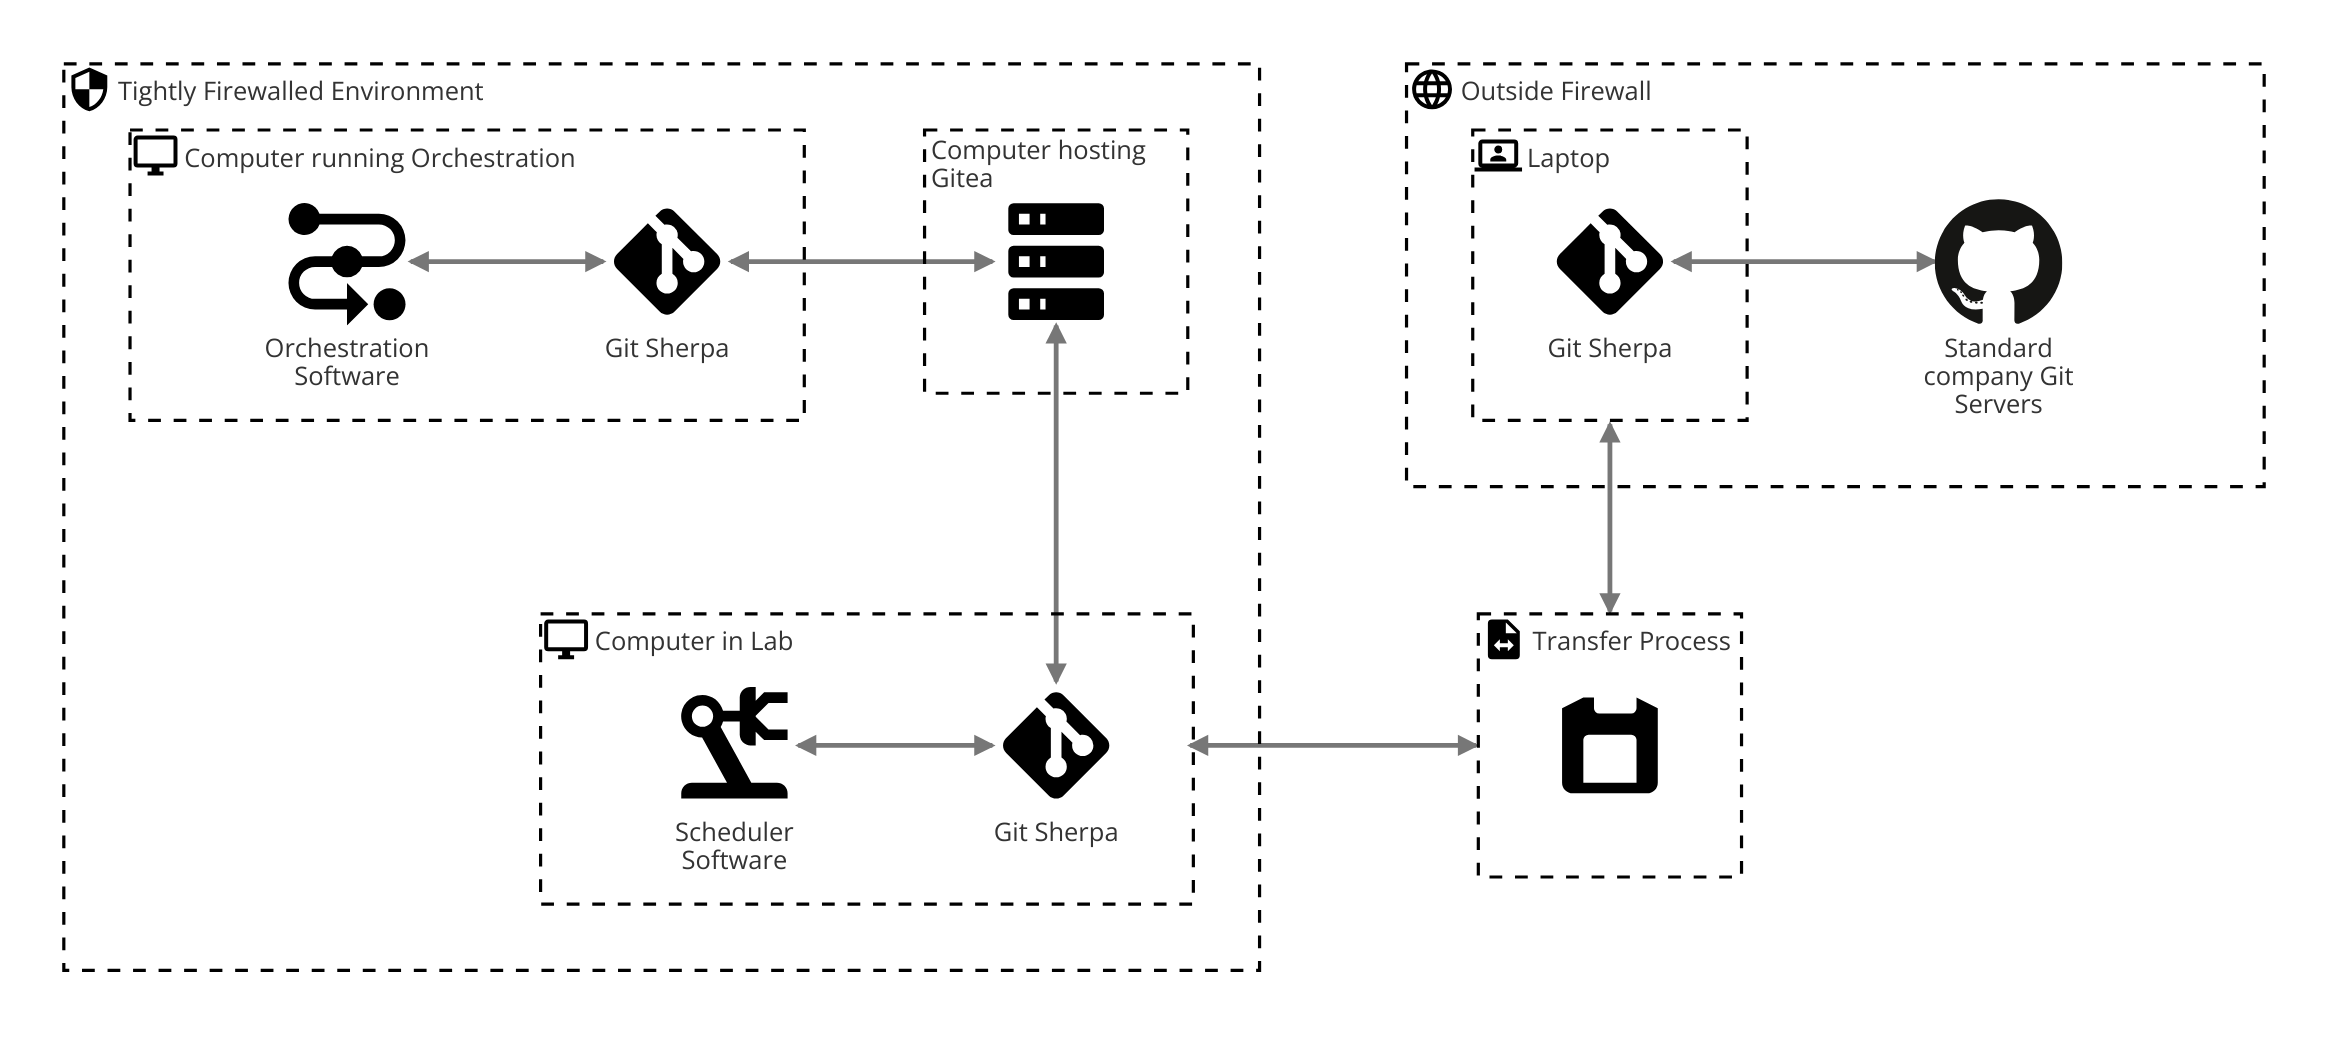
\includegraphics[width=\linewidth,keepaspectratio]{assets/git-architecture.png}
      % If you want a fixed height instead, use:
      % \includegraphics[height=0.62\textheight,keepaspectratio]{assets/my-graphic}
    \end{column}
  \end{columns}

\end{frame}


\begin{frame}[\DefaultVerticalSlideContentAlignment]
  \frametitle{Git Sherpa --- Guiding Users through Git}
    \vskip2ex\begin{overlayarea}{\textwidth}{0.65\textheight}
    \hspace{2cm}{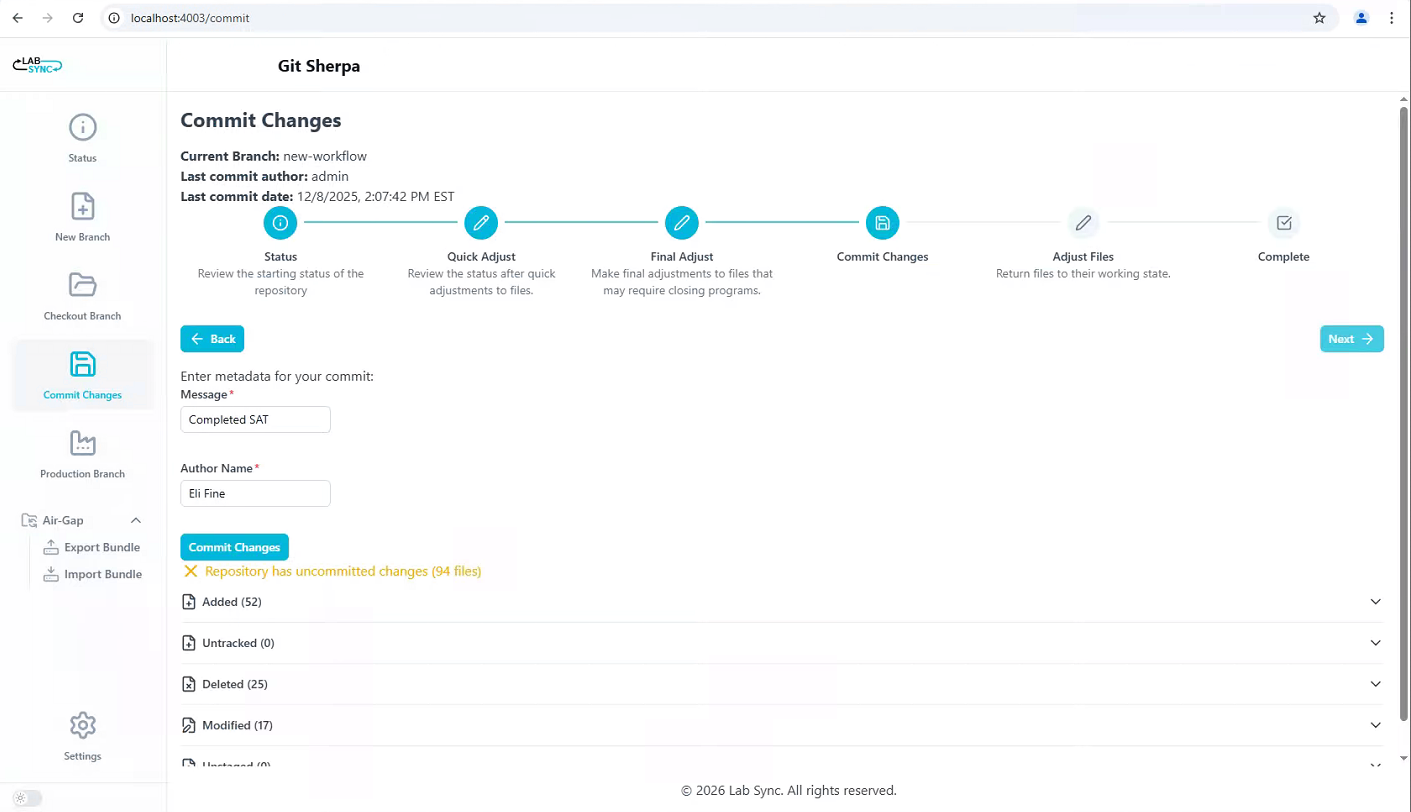
\includegraphics[height=0.65\textheight,keepaspectratio]{assets/commit-light.png}} 
    
  \end{overlayarea}
  
\end{frame}

\begin{frame}[\DefaultVerticalSlideContentAlignment]
  \frametitle{Handling Version Control Challenges for Automation}
  \pause

  \begin{FlushWithFrameTitleItemize}[<+->]
    % \item Challenges
    %       \begin{FlushWithFrameTitleItemize}[<+->]
    %         \item Vendor software does not write to disk until fully closed
    %         \item Vendor software stores some configuration not on disk
    %         \item Various attributes in vendor text files are environment-specific
    %       \end{FlushWithFrameTitleItemize}

    % \item Git Sherpa Solutions
    %       \begin{FlushWithFrameTitleItemize}[<+->]
    %         \item Checks in the workflow if programs are closed
    %         \item Queries vendor software to read/write configuration to disk
    %         \item Makes specified adjustments to files based on environment (lab vs simulation)
    %       \end{FlushWithFrameTitleItemize}
  \item Vendor software does not write to disk until fully closed
          \begin{FlushWithFrameTitleItemize}[<+->]
            \item Check in the workflow if programs are closed

          \end{FlushWithFrameTitleItemize} 
            \item Vendor software stores some configuration not on disk
          \begin{FlushWithFrameTitleItemize}[<+->]
            
            \item Query vendor software to read/write configuration to disk
            
          \end{FlushWithFrameTitleItemize}
    \item Various attributes in vendor text files are environment-specific
          \begin{FlushWithFrameTitleItemize}[<+->]
            \item Make specified adjustments to files when in simulation environment
          \end{FlushWithFrameTitleItemize} 
   
  \end{FlushWithFrameTitleItemize}
  
    \only<8->{\vskip0ex\begin{overlayarea}{\textwidth}{0.2\textheight}
    \hspace{2cm}{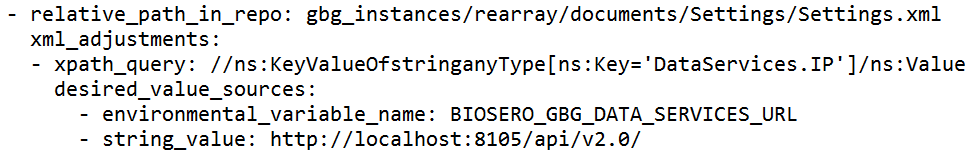
\includegraphics[height=0.2\textheight,keepaspectratio]{assets/adjustment-config.png}}
    
  \end{overlayarea}}\end{frame}

\begin{frame}[\DefaultVerticalSlideContentAlignment]
  \frametitle{Gitea --- Fully Featured Git in the Lab}
  

  \begin{columns}[T,onlytextwidth]
    % Left side: bullet list
    \begin{column}{0.35\textwidth}
        \begin{FlushWithFrameTitleItemize}[<+(1)->]
            \item Pull Requests
            \item Comments/discussions
            \item Diffs of what changed
            \item Branch approval rules
            \item Authentication
          \end{FlushWithFrameTitleItemize}
  \end{column}

    % Right side: graphic
    \begin{column}{0.65\textwidth}
      \vspace{0pt} % helps top-align the graphic with the left column
      \centering
      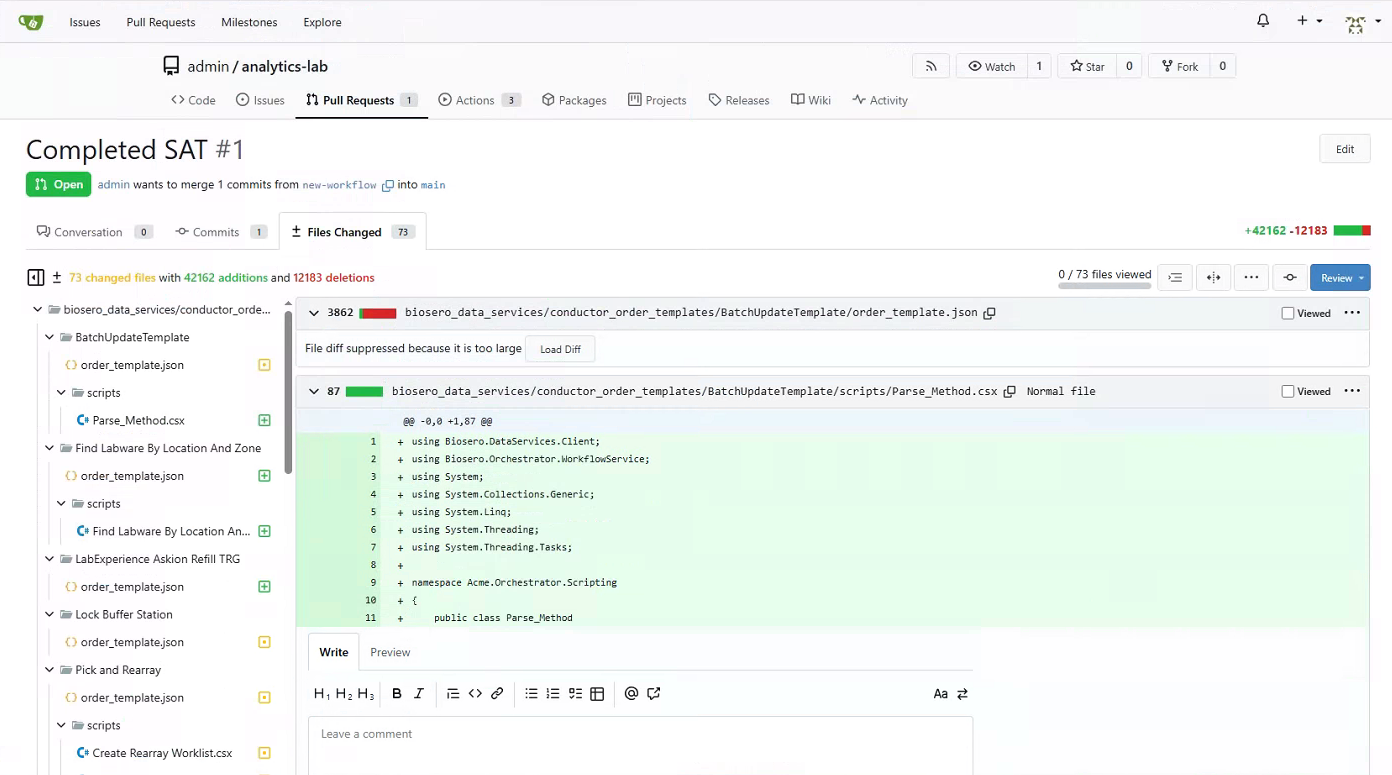
\includegraphics[width=\linewidth,keepaspectratio]{assets/pr-light.png}
      % If you want a fixed height instead, use:
      % \includegraphics[height=0.62\textheight,keepaspectratio]{assets/my-graphic}
    \end{column}
  \end{columns}

\end{frame}


\begin{frame}[\DefaultVerticalSlideContentAlignment]
  \frametitle{Version Control Authentication}
  \pause
  \begin{FlushWithFrameTitleItemize}[<+->]
    \item While wearing PPE doing live work:
  \begin{FlushWithFrameTitleItemize}[<+->]
    \item Git Sherpa uses an API token with no permission to affect Production
    \item No required user-authentication
    \item Text field in Git Sherpa to associate name with commits
    
    
      \end{FlushWithFrameTitleItemize}  
    \item When ready to change Production code:
      \begin{FlushWithFrameTitleItemize}[<+->]
    \item Configurable user-authentication flow (internal username/password within Gitea, Active Directory...)
    \item Pull Requests for any merge into Production branch
    \item Required review and approval of changes
    
      \end{FlushWithFrameTitleItemize}  

\end{FlushWithFrameTitleItemize}  
\end{frame}


\begin{frame}[\DefaultVerticalSlideContentAlignment]
  \frametitle{Conclusions}
  \pause
  \begin{FlushWithFrameTitleItemize}[<+->]
    \item Tightly firewalled networks interfere with historical lab automation practices
    \item Containerized applications can recreate familiar functionality within firewall
    \item Nexus Notifications Center can aggregate alerts via email and API calls
    \item Git Sherpa makes version control approachable with minimal friction
    \item Combining Git Sherpa, Gitea, and Bundles enables version control in the lab synchronized with a simulation environment
    \item Open source approach allows community contributions to expand Git Sherpa's ability to version control additional lab automation software necessitating `custom' interactions

\end{FlushWithFrameTitleItemize}  
\end{frame}



\begin{frame}
  \vfill
  \centering
  {\usebeamerfont{title} Questions? \par}
  \vfill
\end{frame}

\begin{frame}[\DefaultVerticalSlideContentAlignment]
  \frametitle{Version Control Across the Air-gap --- Workflow}
    \vskip2ex\begin{overlayarea}{\textwidth}{0.65\textheight}
    \hspace{2cm}{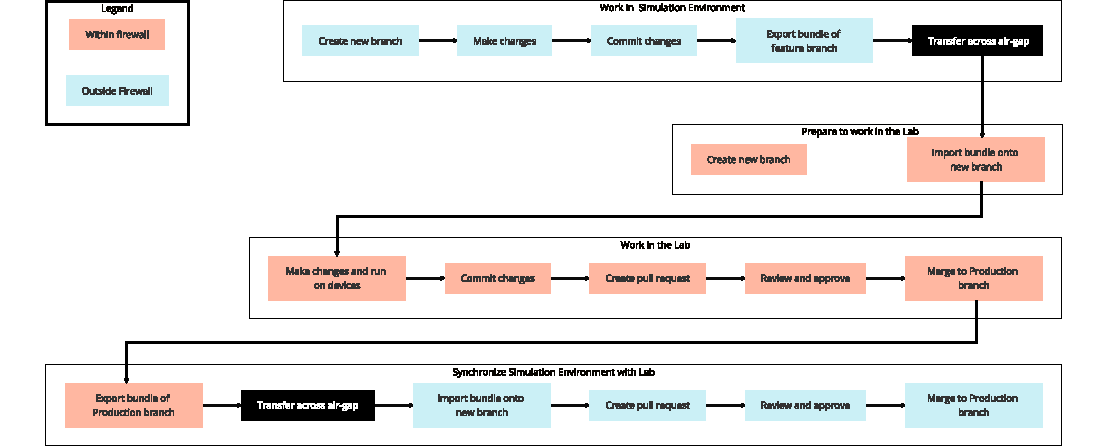
\includegraphics[height=0.65\textheight,keepaspectratio]{assets/git-flow}} 
    
  \end{overlayarea}
  
\end{frame}


\begin{frame}[\DefaultVerticalSlideContentAlignment]
  \frametitle{Future Directions}
  \pause
  \begin{FlushWithFrameTitleItemize}[<+->]
    \item Dot the `i's and cross the `t's with marketing/legal to finish open-sourcing this
    \item Create the ability for users to create their own ``plugins'' for Git Sherpa for placing unusual pieces of lab automation configuration under version control
    \item Enable users to create ``plugins'' for how Nexus Notifications Center forwards alerts to a system within the firewall or through a tunnel to external services

\end{FlushWithFrameTitleItemize}  
\end{frame}

\end{document}
